\documentclass[submission,copyright,creativecommons]{eptcs}
\providecommand{\event}{ML 2014}

\usepackage{graphicx}
\usepackage{xcolor}
\usepackage[fleqn]{amsmath}
\usepackage[hang,flushmargin]{footmisc} 
\usepackage{graphics} 
\usepackage{stmaryrd}
\usepackage{amsthm}
%\usepackage{breakurl}

% =================================================================================================

\newcommand{\langl}{\begin{picture}(4.5,7)
\put(1.1,2.5){\rotatebox{60}{\line(1,0){5.5}}}
\put(1.1,2.5){\rotatebox{300}{\line(1,0){5.5}}}
\end{picture}}
\newcommand{\rangl}{\begin{picture}(4.5,7)
\put(.9,2.5){\rotatebox{120}{\line(1,0){5.5}}}
\put(.9,2.5){\rotatebox{240}{\line(1,0){5.5}}}
\end{picture}}

\newcommand{\lang}{\begin{picture}(5,7)
\put(1.1,2.5){\rotatebox{45}{\line(1,0){6.0}}}
\put(1.1,2.5){\rotatebox{315}{\line(1,0){6.0}}}
\end{picture}}
\newcommand{\rang}{\begin{picture}(5,7)
\put(.1,2.5){\rotatebox{135}{\line(1,0){6.0}}}
\put(.1,2.5){\rotatebox{225}{\line(1,0){6.0}}}
\end{picture}} 

\mathindent=1em

\definecolor{cmtclr}{rgb}{0.0,0.6,0.0}
\definecolor{kvdclr}{rgb}{0.0,0.0,0.6}
\definecolor{strclr}{rgb}{0.5,0.1,0.0}
\definecolor{prepclr}{rgb}{0.0,0.0,0.0}

\newcommand{\sem}[1]{\llbracket #1 \rrbracket}
\newcommand{\ignp}{\_\kern-.5ex\_\kern-.5ex\_ }
\newcommand{\kvd}[1]{\textnormal{\textcolor{kvdclr}{\sffamily #1}}}
\newcommand{\str}[1]{\textnormal{\textcolor{strclr}{\ttfamily "#1"}}}
\newcommand{\ident}[1]{\textnormal{\sffamily #1}}
\newcommand{\lident}[1]{\textnormal{\sffamily 
  \`{}\hspace{-0.25em}\`{}\hspace{-0.1em}#1\`{}\hspace{-0.25em}\`{}}}
\newcommand{\cmt}[1]{\textit{\sffamily\textcolor{cmtclr}{#1}}}
\newcommand{\narrow}[1]{\hspace{-0.75em} #1 \hspace{-1.25em}~}

\newtheorem*{theorem*}{Theorem}

% =================================================================================================

\title{In the Age of Web:\\
  \textnormal{\LARGE Typed Functional-First Programming Revisited}}

\author{Tomas Petricek
\institute{University of Cambridge, UK}
\email{tomas@tomasp.net}
\and
Don Syme
\institute{Microsoft Research Cambridge, UK}
\email{don.syme@microsoft.com}
}
\def\titlerunning{In the Age of Web: Typed Functional-First Programming Revisited}
\def\authorrunning{T. Petricek, D. Syme}
\begin{document}
\maketitle

% =================================================================================================

\begin{abstract}
% What is the problem
Most programming languages were designed before the age of web.
% Why is this a problem
This matters because the web changes many assumptions that typed functional language designers take 
for granted. For example, programs do not run in a closed word, but must instead interact with 
(changing and likely unreliable) services and data sources, communication is often asynchronous 
or event-driven, and programs need to interoperate with untyped environments.

% What is my solution
In this paper, we present how F\# language and libraries face the challenges posed by the web.
Technically, this comprises using \emph{type providers} for integration with external information 
sources and for integration with untyped programming environments, using \emph{lightweight 
meta-programming} for targeting JavaScript and \emph{computation expressions} for writing 
asynchronous code.

% Why does the solution matter
In this inquiry, the holistic perspective is more important than each of the features in isolation.
We use a practical case study as a starting point and look how F\# language and libraries approach 
the challenges posed by the web. The specific lessons learned are perhaps less interesting than 
our attempt to uncover hidden assumptions that no longer hold in the age of web.
\end{abstract}

                                                     

% =================================================================================================
%
%                         #                #           
%   #       #               #            #               
%   # # #  #### # #  ##   ### #  #  ### #### #  ##  # #  
%   # ## #  #   ### #  # #  # #  # #     #   # #  # ## # 
%   # #  #  #   #   #  # #  # #  # #     #   # #  # #  # 
%   # #  #  #   #   #  # #  # #  # #     #   # #  # #  # 
%   # #  #  #   #   #  # # ## # ## #     #   # #  # #  # 
%   # #  #   ## #    ##   # #  # #  ###   ## #  ##  #  # 
%                                                    
% =================================================================================================


\section{Introduction}

Among the ML family of languages, F\# often takes a pragmatic approach and emphasizes ease of use
and the ability to integrate with its execution environments\footnote{Historically, this applied 
to the .NET runtime, but the same applies to integrating with JavaScript in the web context.} over 
other aspects of language design. If you use the F\# language as ML, you get most of the good 
well-known properties of ML\footnote{For example, F\# does not require type annotations when used 
as ML, but requires them when used with .NET objects.}. However, F\# leaves enough \emph{holes} that
let you use it \emph{not} as ML. This is the space that we explore in this paper.

This additional flexibility makes it possible to use F\# in ways that break the common assumptions
that are often taken for granted in languages such as ML and Haskell\footnote{In a way, we are trying
to uncover the hidden assumptions of the functional programming \emph{research programme} that are
normally ``\emph{rendered unfalsifiable by the methodological decisions of its protagonists}.'' 
(Lakatos \cite{philosophy-lakatos}, quoted by Chalmers \cite{philosophy-thing})}. The focus on 
the web directs our inquiry and provides an angle for reconsidering such assumptions. 

Perhaps the most remarkable assumption is the idea that programs fundamentally operate in a closed
world. Although we have learned how to perform FFI and I/O \cite{haskell-ffi,haskell-imperative},
those are treated as dealing with the ``dirty real world''. For a practical solution, we argue that
we need to go much further, but deeper integration with (untyped) JavaScript libraries and (evolving) 
services inevitably breaks strict type safety requirements.

We do not claim that the F\# approach is the only possible. Rather, this paper should be seen
as a programming language experiment \cite{philosophy-pl} or an empirical observation of the 
approach used by the F\# community. We aim to provide an intriguing exploration of hidden assumptions 
and present what can be achieved using a combination of F\# features. We do so by starting with 
a simple, yet real-world problem and then exploring a solution. More specifically, the contributions 
of this position paper are:

\begin{itemize}
\item We present a case study (Section~\ref{sec:case}) showing how a combination of numerous
  F\# language features can be used for the development of modern web applications. This
  is not a toy demonstration, but an example of how F\# is used in the industry.

\item We discuss how type providers make it possible to access external information sources
  in web applications (Section~\ref{sec:tp-data}) and integration with (untyped) programming
  environments such as the JavaScript ecosystem (Section~\ref{sec:tp-lang}). 

\item We show how F\# approaches the problem of compilation to JavaScript using a library 
  called FunScript (Section~\ref{sec:js-meta}), outlining important practical concerns such as 
  interoperability (Section~\ref{sec:js-lib}) and asynchronous execution (Section~\ref{sec:js-async}).

\item Throughout the paper, we discuss how the age of the web breaks the assumptions commonly 
  taken as granted in typed functional programming. We revisit the notion of type safety
  in the context of web (Section~\ref{sec:tp-relative}) and the notion of fixed language 
  semantics (Section~\ref{sec:js-relative}).
\end{itemize}

\noindent
In the first part of the paper (Section~\ref{sec:case}), we present a case study of using 
F\# for web development. The rest of the paper (Section~\ref{sec:tp} and \ref{sec:js}) discusses 
the arising issues in more depth. The source code and running demo for the case study is available 
at: \url{http://funscript.info/samples/worldbank}



% =================================================================================================
%                                                  
%                                            #      
%     ###                   ###  #           #      
%    #     ##    ##  ##    #    #### #  #  ### #  # 
%   #        #  #   #  #   #     #   #  # #  # #  # 
%   #      ###  ##  ####    ##   #   #  # #  # #  # 
%   #     #  #   ## #         #  #   #  # #  # #  # 
%    #    #  #    # #         #  #   # ## # ##  ##  
%     ###  ## # ##   ###   ###    ##  # #  # #  ##  
%                                               #   
%                                              ##   
% =================================================================================================


\section{Case Study: Web-based data analytics}
\label{sec:case}
In this case study, we develop a web application shown in Figure~\ref{fig:wb}, which lets the
user compare university enrollment in a number of selected countries and regions around the world. 
The resulting application runs on the client-side (as JavaScript) and fetches data dynamically 
from the World Bank \cite{data-wb-schter}.

The application is an example of a web page that could be built in the context of data journalism 
\cite{dj-handbook}. As such, it is relatively simple, works with just a single data source and 
uses a concrete indicator and a hard-coded list of countries \emph{i.e.}~to illustrate a point 
made in an accompanying article.

% -------------------------------------------------------------------------------------------------

\subsection{Accessing World Bank data with type providers}

To access the university enrollment information, we first obtain a list of countries using the 
World Bank type provider from the F\# Data library \cite{fsharp-data}. The type provider exposes 
the individual countries as members of an object (the notation \lident{Country Name} is used for 
identifiers with spaces):
%
\begin{equation*}
\begin{array}{l}
 \kvd{type}~\ident{WorldBank}~=~\ident{WorldBankData}\langl\ident{Asynchronous}=\kvd{true}\rangl
 \\[0.5em]
 \kvd{let}~\ident{data}~=~\ident{WorldBank.GetDataContext}() \\
 \kvd{let}~\ident{countries}~= \\
 \quad~\lbrack~~ \ident{data.Countries.}\lident{European Union} \\
 \qquad   \ident{data.Countries.}\lident{Czech Republic} \\
 \qquad   \ident{data.Countries.}\lident{United Kingdom} \\
 \qquad   \ident{data.Countries.}\lident{United States} ~\rbrack 
\end{array}
\end{equation*}
%
The type provider connects to the World Bank and obtains a list of countries at 
\emph{compile-time} and at \emph{edit-time} (when using auto-completion in an editor).
This means that the list is always up-to-date and we get a compile time error when accessing 
a country that no longer exists (a property discussed in Section~\ref{sec:tp-data}).

On the first line, we provide a static parameter \ident{Asynchronous}. Static parameters are 
resolved at compile-time (or edit-time). Here, we specify that the exposed types for accessing 
information should support only non-blocking functions. This is necessary for a web-based 
application, because JavaScript only supports non-blocking calls (using callbacks) to fetch the data. 

% =================================================================================================

\begin{figure}[!t]
\hspace{3em} 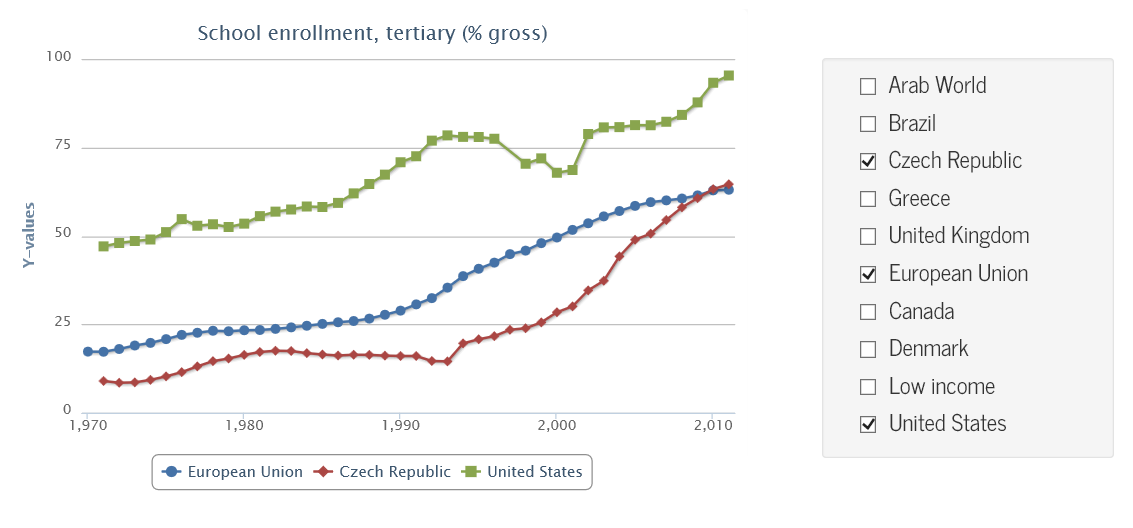
\includegraphics[width=35em]{worldbank.png}
\caption{Case study -- web application for comparing university enrollment in the world}
\label{fig:wb}
\end{figure}

% =================================================================================================

\subsection{Interoperating with JavaScript libraries}
To run the sample application on the client-side we use FunScript \cite{fsharp-funscript}, which 
is a library that translates F\# code to JavaScript (Section~\ref{sec:js}). Aside from 
running as JavaScript, we also want to use standard JavaScript libraries, including jQuery for DOM 
manipulation and Highcharts for charting. FunScript comes with a type provider that imports 
TypeScript \cite{ms-typescript} definitions for JavaScript libraries:
%
\begin{equation*}
\begin{array}{lll}
 \kvd{type}~\ident{j}~&\narrow{=}&~\ident{TypeScript}\langl\str{jquery.d.ts}\rangl \\
 \kvd{type}~\ident{h}~&\narrow{=}&~\ident{TypeScript}\langl\str{highcharts.d.ts}\rangl \\
\end{array}
\end{equation*}
%
The \textcolor{strclr}{\ttfamily d.ts} files are type annotations created for the TypeScript language.
Here, the type provider mechanism lets us leverage an existing effort for annotating common JavaScript 
libraries. The type provider analyses those definitions and maps them into F\# types named \ident{j} and 
\ident{h} that contain statically typed functions for calling the JavaScript libraries (we will use
them shortly). The file names are static parameters (same as \ident{Asynchronous} earlier) and are 
statically resolved and accessed at compile-time or edit-time.

Importing types for JavaScript libraries into the F\# type system has interesting implications, 
because the TypeScript language does not have the traditional type safety property \cite{ms-safets}.
We return to this topic in Section~\ref{sec:tp-lang}. Next, we generate checkboxes that appear on the 
right in Figure~\ref{fig:wb}:
%
\begin{equation*}
\begin{array}{lll}
 \kvd{let}~\ident{jQuery}~\ident{command}~=~\ident{j.jQuery.Invoke}(\ident{command}) 
 \\[0.5em]
 \kvd{let}~\ident{infos}~=~\ident{countries}~|\rang~\ident{List.map}~(\kvd{fun}~\ident{country}~\rightarrow \\
 \quad \kvd{let}~\ident{inp}~=~\ident{jQuery}(\str{<input>})\ident{.attr}(\str{type}, \str{checkbox}) \\
 \quad \ident{jQuery}(\str{\#panel})\ident{.append}(\ident{inp})\ident{.append}(\ident{country.Name}) \\
 \quad \ident{country.Name}, \ident{country.Indicators}, \ident{el}) \\
\end{array}
\end{equation*}
%
To manipulate the DOM (Document Object Model), we are using the jQuery library in a way that is
very similar to code that one would write in JavaScript. We define a helper function \ident{jQuery}
(hiding some of the complexities of the mapping) and use it to create the \str{<input>} element and
specify its attributes. Note that members like \ident{append} and \ident{attr} are standard 
jQuery patterns. The compiler sees them as ordinary object members. When writing code using F\# editors
based on the F\# Compiler Service \cite{fsharp-fcs}, they also appear in the auto-complete list.

Although the jQuery library is not perfect, it is a de facto standard in web development. The 
FunScript type provider makes it possible to integrate with it painlessly without explicitly 
specifying any FFI interface and without manual wrapping (see also Section~\ref{sec:js-lib}). 

Note that we use a standard F\# function \ident{List.map} to iterate over the countries. This has 
a side-effect of creating the HTML elements, but it also returns a new list. The result is a list 
of $\ident{string}\ast\ident{Indicators}\ast\ident{jQuery}$ values representing the country name,
its indicators (for accessing the World Bank data) and the created DOM object representing the
checkbox.

% -------------------------------------------------------------------------------------------------

\subsection{Loading data and updating the user interface}
\label{sec:case-loading}

The main part of the sample program is a function \ident{render} that asynchronously fetches 
data for selected countries and generates a chart. To keep the code simple, we iterate over the 
\ident{infos} list from the previous section and load data for countries one by one:
%
\begin{equation*}
\begin{array}{lll}
 \kvd{let}~\ident{render}~()~=~\ident{async}~\{ \\
 \quad \kvd{let}~\ident{head}~=~\str{School enrollment, tertiary (\% gross)} \\
 \quad \kvd{let}~\ident{o}~=~\ident{h.HighchartsOptions}() \\
 \quad \ident{o.chart} \leftarrow \ident{h.HighchartsChartOptions}(\ident{renderTo}=\str{plc}) \\
 \quad \ident{o.title} \leftarrow \ident{h.HighchartsTitleOptions}(\ident{text}~=~\ident{head}) \\
 \quad \ident{o.series} \leftarrow \lbrack| ~ |\rbrack
 \\[0.5em]   
 \quad \kvd{for}~\ident{name},~\ident{ind},~\ident{check}~\kvd{in}~\ident{infos}~\kvd{do}\\
 \qquad   \kvd{if}~\ident{unbox}\langl \ident{bool} \rangl~(\ident{check.is}(\str{:checked}))~\kvd{then} \\
 \qquad\quad     \kvd{let!}~\ident{v}~=~\ident{ind.}\lident{School enrollment, tertiary (\% gross)} \\
 \qquad\quad     \kvd{let}~\ident{data}~=~\ident{vals}~
                   |\rang~\ident{Seq.map}~(\kvd{fun}~(\ident{k}, \ident{v})~\rightarrow \lbrack|~\ident{number~k};~\ident{number~v} ~|\rbrack)~
                   |\rang~\ident{Array.ofSeq} \\
 \qquad\quad     \ident{opts.series.push}(\ident{h.HighchartsSeriesOptions}(\ident{data}, \ident{name})) ~\}
\end{array}
\end{equation*}
%
Although the function looks like ordinary code, it is wrapped in the $\ident{async}~\{\ldots\}$ 
block, which is an F\# computation expression \cite{fsharp-zoo}. The F\# compiler performs 
de-sugaring similar to the CPS transformation and interprets keywords such as \kvd{let!} and 
\kvd{for} using special operations (monadic bind and other). The \ident{async} identifier 
determines that we are writing asynchronous workflow \cite{fsharp-async} that makes it 
possible to include non-blocking calls in the block.

Here, the non-blocking call is done when accessing the \lident{School enrollment, tertiary (\% gross)} 
indicator using the \kvd{let!} keyword. The indicator is a member (with a name wrapped in 
back-ticks to allow spaces) exposed as an asynchronous computation by the World Bank type provider.
The rest of the code is mostly dealing with the DOM and the Highcharts library using the API 
imported by FunScript -- we iterate over all checkboxes and generate a new chart series for each 
checked country. 

Two notable points here are that \ident{async} translated to JavaScript is restricted to a single 
thread, which is not the case for ordinary F\# code (Section~\ref{sec:js-async}) and that the 
\ident{HighchartOptions} object preserves some of the underlying JavaScript semantics 
(Section~\ref{sec:js-lib}). Finally, the last part of the example code registers event handlers that 
redraw the chart when checkbox is clicked:
%
\begin{equation*}
\begin{array}{lll}
 \kvd{for}~\ignp, \ignp,~\ident{check}~\kvd{in}~\ident{infos}~\kvd{do} \\
 \quad \ident{check.click}(\kvd{fun}~\ignp~\rightarrow \ident{Async.StartImmediate}(\ident{render}()))
\end{array}
\end{equation*}
%
The \ident{click} operation (exposed by jQuery) takes a function that should be called when the 
event occurs. Calling it is a side-effectful operation that registers the handler. As \ident{render} 
is an asynchronous operation, we invoke it using the \ident{StartImmediate} primitive from the 
F\# library, which starts the computation without waiting for the result (the only way to start
a non-blocking operation in JavaScript).

% -------------------------------------------------------------------------------------------------

\subsection{Learning from the case study}

The case study shows that we can develop a simple interactive data visualization (that could
be built, for example, by data journalists) in less than 30 lines of F\# code. The code uses 
many typical functional patterns (lists, first-class functions, data types), but also uses features
that are more specific to F\# (type providers, objects, computation expressions). 

Before analysing the interesting aspects of this case study, we briefly review the points that we 
find appealing and points that many would find unappealing or, at least, peculiar. First, the 
appealing points:

\begin{itemize}
\item The ML approach to types and type inference can be extended from (closed-world) data types 
  to (open-world) types for rich information sources such as World Bank. The sample code is 
  fully statically typed without explicit type annotations. Critically, types are also used for 
  exploratory programming when finding indicators using auto-complete in an editor.

\item The case study demonstrates that core ML programming style can be used in the context of
  client-side (JavaScript) web development. We used functional lists, standard higher-order 
  functions such as \ident{List.map} in much the same way as when writing ordinary F\#.

\item In addition to standard functional constructs, we were also able to reuse F\# asynchronous
  workflows to write non-blocking code that requests data from a web service (World Bank), 
  rather than using error-prone explicit callbacks that are common in JavaScript.

\item Finally, we were able to painlessly call Highcharts and jQuery. No explicit wrapping or 
  importing of individual functions and types was necessary. Moreover, despite the differences between 
  the F\# and JavaScript object model, the code is close to idiomatic F\#.
\end{itemize}

\noindent
Now, the following list looks at the aspects that appear unappealing or peculiar, especially when 
coming from the traditional functional programming background:

\begin{itemize}
\item The World Bank type provider lifts information about countries to the type level. As a result,
  we can easily write $\ident{data.Countries.}\lident{Czech Republic}$, but if Czech Republic is
  removed from the World Bank (and becomes Czechoslovakia again), the code will no longer compile
  (Section~\ref{sec:tp-data}).

\item The TypeScript language is unsound due to covariant generics \cite{ms-safets}. Thus
  importing types from TypeScript definitions introduces a potential unsoundness into the F\# 
  code (Section~\ref{sec:tp-lang}).

\item When compiling F\# to JavaScript, the FunScript library does not fully preserve the 
  semantics of F\#. For example, numerical types behave as in JavaScript (Section~\ref{sec:js-meta})
  and asynchronous workflows run on a single thread (Section~\ref{sec:js-async}).
\end{itemize}

\noindent
The most notable observation about the above points is that there is often both a positive and
a negative side: we can nicely access World Bank data, but it affects soundness properties;
we can interoperate with JavaScript libraries, but we can not fully hide undesirable JavaScript 
behaviours.

The aim of this paper is not to make value judgements and argue what is better. Using the case
study as a basis, we claim that the outlined approach is \emph{one possible} and that it
\emph{works in practice}. In the rest of the paper, we give more details about the most important 
aspects of the approach and discuss alternatives.

                                                  

% =================================================================================================
%
%                                            #    # 
%     ##                    #     #          #    # 
%    #  #  # #   ##  # #    #  #  #  ##  # # #  ### 
%   #    # ## # #  # ## #   #  #  # #  # ### # #  # 
%   #    # #  # #### #  #   # # # # #  # #   # #  # 
%   #    # #  # #    #  #    #   #  #  # #   # #  # 
%    #  #  #  # #    #  #    #   #  #  # #   # # ## 
%     ##   ###   ### #  #    #   #   ##  #   #  # # 
%          #                                        
%          #                                        
% =================================================================================================


\section{Integrating with the open world}
\label{sec:tp}

Type providers \cite{fsharp-typeprov} is a mechanism for integrating external components into a 
statically typed programming language. Such components include information sources (such as World
Bank), other environments (here, JavaScript libraries via TypeScript), but type-providers can 
also be used for limited meta-programming (the \ident{Asynchronous} parameter can be seen as
a form of meta-programming).

% -------------------------------------------------------------------------------------------------

\subsection{How type providers work and fail}
\label{sec:tp-def}

In technical terms, type providers are libraries that are loaded by the compiler (and editor)
and are executed at compile-time (or edit-time). A type provider builds information about types
it provides and makes those available to the compiler. It is worth noting that this is done lazily,
so the type provider does not need to provide types for the entire information space at once.

In terms of programming language theory, type providers can be easily explained anecdotally. 
They change the starting point for a type-checking of a program as follows:
%
\begin{equation*}
\hspace{8em}
\begin{array}{rclll}
 \emptyset &\narrow{\vdash}& e : \tau 
    &\qquad& (\textit{classical, or closed-world})\\
 \pi~(
\includegraphics[width=1em,trim=0 1.5em 0 0]{earth.png})  &\narrow{\vdash}& e : \tau
    &\qquad& (\textit{type providers, or open-world})
\end{array}
\end{equation*}
%
Rather than starting the type-checking with an empty context, we start type-checking with a
context containing a \emph{projection} of some information from the world. In this paper, we do not
attempt to formalize type providers, so we avoid the question of what, formally, is the world here.
However, this analogy is useful for understanding how type providers work and how they can go wrong:

\begin{itemize}
\item \emph{Type provider failure.} 
  The projection (a type provider) is implemented in F\# and can fail (for example, if internet
  is required but unavailable). However, when it succeeds, it generates a valid F\# code and so 
  unchecked compilation errors cannot happen.

\item \emph{Runtime failure.}
  When the world changes and we \emph{run} the program, we may get a runtime exception. It is
  expected that the provided code will not fail as long as certain assumptions are satisfied (for
  example, countries are not removed from a database). But if the world changes and the assumptions
  no longer hold, the provided code may fail with a runtime exception.

\item \emph{Recompilation failure.} 
  When the world changes and we \emph{recompile} the program, the result of the projection can
  differ and so we may not be able to type-check code that used to type-check. This can be seen as
  negative aspect, but there is a clear benefit -- it means we discover an error that would happen
  at runtime earlier, that is during recompilation.
\end{itemize}

\noindent
The above points are \emph{general} points about type providers. In this paper, we are more interested
in the \emph{specific} type providers used in the case study. We look at the World Bank and TypeScript
type providers in the following two sections. When discussing type providers, we need to look at 
how the provider (or the projection $\pi$) works and what assumptions it makes about the world. 
That is, what world changes cause the provided type to change and what world changes cause a 
runtime exception. 

% -------------------------------------------------------------------------------------------------

\subsection{Integrating with World Bank data}
\label{sec:tp-data}

The World Bank provider \cite{fsharp-data} is a type provider for a specific data source -- it has 
been designed specifically for World Bank data. This contrasts with F\# Data type providers for 
working with CSV, XML and JSON data that take sample or schema as parameter and can thus be used 
with files of any structure.

\subsubsection{The World Bank type provider}

The projection implemented by the type provider generates a type called \ident{Countries} that contains 
countries (and regions) as members. Each member returns a value of type \ident{Indicators} that is
also generated and contains all indicators as members. Note that the type provider generates just 
these two types -- in particular, it does not generate a new type for each country. This would be an 
interesting option if we could check what indicators are available for a given country.

The type provider builds the structure of the provided types, but the provided types are \emph{erased} 
during compilation and replaced with runtime implementation. For the World Bank type provider, the 
erasure works as follows:
%
\begin{equation*}
\begin{array}{lcl}
 \sem{~\ident{data.}\lident{Czech Republic}~} &=&
   \ident{data.GetCountries}().\ident{GetCountry}(\str{CZE}) \\
 \sem{~\ident{cz.}\lident{School enrollment, tertiary (\% gross)}~} &=&
   \ident{cz.AsyncGetIndicator}(\str{SE.TER.ENRR})
\end{array}
\end{equation*}
%
The underlying operations (\ident{GetCountry}, \ident{GetCountries} and \ident{AsyncGetIndicator})
are operations of an underlying runtime library (which is a normal non-provided library). This is
a typical pattern -- type providers generally produce a light layer on top of a rich runtime library.

An important point here is that the type provider uses the \emph{name} of a country or an indicator
for the member name, but at runtime, it uses a \emph{code} of the country or the indicator. This has
interesting implications for the safety properties, as discussed in the next section.

\subsubsection{Safety properties of the type provider}

Now that we know how the World Bank type provider generates the types and the runtime code, we can 
look at the assumptions it makes about the world and in which cases it encounters one of the failures
defined in Section~\ref{sec:tp-def}.

\begin{itemize}
\item If you are offline when using the type provider (compiling or editing), the type provider will
  not be able to obtain the list of countries or indicators. This is an example of \emph{type provider
  failure}. In case of World Bank, this is partly prevented by caching of the schema, but internet
  access is required when using the provider for the first time.

\item An interesting case is when a country or indicator is renamed. In that case, compiled code
  using the World Bank type provider will continue to work (there is no \emph{runtime failure}), 
  because the lookup uses the country or the indicator code. However, recompilation will fail
  as the member name (which appears in the source code) will be different.

\item Finally, if a country or indicator completely disappears, we will get \emph{runtime failure}
  when running existing compiled code and \emph{recompilation failure}. here, the \emph{recompilation
  failure} is a useful indicator that the assumptions made by our code have been violated by
  the data source.
\end{itemize}

\noindent
When contrasted with the traditional view of safety in ML family of languages, the World Bank 
type provider certainly relaxes the usual safety conditions. However, this is not the case when 
compared with standard developer practices. In particular, if we wrote 
$\ident{data.GetCountries}().\ident{GetCountry}(\str{CZE})$ by hand, the \emph{runtime failure}
behaviour would be the same, but we would lose the useful \emph{recompilation failure}. The following
section discusses this (and other) alternatives.

\subsubsection{Discussion of alternatives}

There are two main alternatives that are worth discussing. First, how would the code look if 
we did not use any type provider. Second, what are alternative designs for the World Bank type 
provider and how would such alternatives change the safety properties. 

\vspace{-1em}
\paragraph{Accessing countries without type providers.} First, consider how would we write the code to obtain a list
of countries without using the World Bank type provider. Assuming we want only the countries and
regions in Figure~\ref{fig:wb}, we could specify the country codes and then obtain the country objects:
%
\begin{equation*}
\begin{array}{l}
 \kvd{let}~\ident{data}~=~\ident{WorldBank.GetDataContext}() \\
 \kvd{let}~\ident{countryCodes}~=~\lbrack~\str{EU},~\str{CZE},~\str{GBP},~\str{USA}~\rbrack \\
 \kvd{let}~\ident{countries}~=~\ident{countryCodes}~|\rangl~\ident{List.map}~(\ident{data.GetCountries}().\ident{GetCountry})
\end{array}
\end{equation*}
%
The motivation for the case study was a data journalism application with a transparent logic
that is easy to understand (and perhaps even modify). The type provider certainly achieves these
goals better -- a country can be added just by looking through an auto-complete list and we do not
need to know its code or exact name. However, if we wanted to list all countries in a region, then
the World Bank type provider would not be helpful. 

As for the safety properties, as discussed earlier, using explicit country codes has the same
runtime properties as using the type provider. This could be avoided by listing all countries in
a given region (or, according to another rule), but that is solving a different problem. 

In summary, the World Bank type provider fits a specific niche that we were exploring in the case 
study. That is, when we want to create an information analysis that accesses specific data from
an information source. With rising popularity of data journalism and Open Government Data
initiatives, we argue that this is an important problem domain. Here, we first specify the country 
codes and then obtain the country objects.

\vspace{-1em}
\paragraph{Providing safer data accessors.} 
The \emph{recompilation failure} when a country is removed from the dataset is an indication that
code would not behave as expected as runtime and so we find it useful. The problematic case is 
a \emph{runtime failure} when a country is removed after the program is compiled. One way to 
avoid this error would be to change the type of the provided members like
\ident{data.}\lident{Czech Republic} from \ident{Country} to \ident{Country~option}. 

However, that is only shifting the burden of error handling from the library to the user. If the
author of the application does not intend to handle errors (for example, by skipping missing data),
they would have to write the following:
%
\begin{equation*}
\begin{array}{l}
 \kvd{let}~\ident{optCountries}~= \\
 \quad~\lbrack~~ \ident{data.Countries.}\lident{European Union} \\
 \qquad   \ident{data.Countries.}\lident{Czech Republic} \\
 \qquad   \ident{data.Countries.}\lident{United Kingdom} \\
 \qquad   \ident{data.Countries.}\lident{United States} ~\rbrack 
\\[0.5em]
 \kvd{let}~\ident{countries}~=\\
  \quad \ident{optCountries}~|\rangl~\ident{List.map}~(\kvd{fun}~\ident{countryOpt}~\rightarrow \\
  \qquad \kvd{match}~\ident{countryOpt}~\kvd{with}~\ident{Some~c}~\rightarrow~\ident{c}~|~\ignp~\rightarrow 
    \ident{failwith}~\str{Country does not exist!})
\end{array}
\end{equation*}
%
For the purpose of our case study, providing option types would only make the code more complex.
However, if we wanted to handle errors more gracefully, then option types would be a better 
alternative. Note, however, that we can still handle exceptions using $\kvd{try}~\ldots~\kvd{with}$.

Whether using option types is more desirable or not often depends on the use case (how we
want to handle errors) and reliability of the data source (countries do not disappear often).
This alternative can be supported by adding a static parameter to the type provider (like
$\ident{Asynchronous}=\kvd{true}$). For example, the CSV type provider from F\# Data has a 
parameter \ident{AssumeMissingValues} that serves exactly this purpose.

\vspace{-1em}
\paragraph{Accessing data ``as of time''.} 
So far, we discussed how to mitigate the problems caused by the fact that the open world changes.
Can we make the world \emph{not} change? This is a sensible question for some data sources
(although not for the World Bank). For example Freebase \cite{google-freebase} supports the 
notion of ``as of time''. When calling Freebase with the \ident{as\_of\_time} parameter, the API
returns data and meta-data that was present at the specified date.

This would be a desirable option for our case study -- if we want to illustrate point made 
by an article, the accompanying application could use data available at the time when the 
article was written. However, this feature relies on the ability of the data source (not all
services have this), or on the possibility to create local snapshots (difficult for large data
sources).

% -------------------------------------------------------------------------------------------------

\subsection{Integrating with JavaScript libraries}
\label{sec:tp-lang}

Type providers are often described as a technique that simplifies data access. The TypeScript
type provider shows that there is a broader range of uses, including integration between different
programming languages. Another example of type provider for language integration is the R
provider \cite{fsharp-rprovider} which imports packages and functions of the statistical 
environment R.

\subsubsection{The TypeScript type provider}
The projection implemented by the TypeScript type provider imports interface definitions in the
\str{.d.ts} format specified by TypeScript \cite{ms-typescript}. This is a format of type 
annotations for JavaScript libraries. The following example is an excerpt from the \str{jquery.d.ts}
file that describes the \ident{jQuery} value and the \ident{attr} method used in our example:
%
\begin{equation*}
\begin{array}{l}
 \kvd{declare var}~\ident{jQuery}~:~\ident{JQueryStatic}; 
\\[0.5em]
 \kvd{interface}~\ident{JQueryStatic}~\{ \\
 \quad (\ident{selector}: \kvd{string}, \ident{context?}: \kvd{any}):~\ident{JQuery}; \\
\} 
\\[0.5em]
\kvd{interface}~\ident{JQuery}~\{ \\
\quad \ident{attr}(\ident{attributeName}~:~\kvd{string}):~\kvd{string}; \\
\quad \ident{attr}(\ident{attributeName}~:~\kvd{string},~\ident{value}~:~\kvd{any}):~\ident{JQuery}; \\
\}
\end{array}
\end{equation*}
%
The example demonstrates a number of typical problems that arise when using type providers for
language interoperation. Not all TypeScript language constructs have direct equivalent in F\# and 
the TypeScript type provider needs to map them to other constructs that are available:
%
\begin{itemize}
\item The interface file defines \ident{jQuery} as a global variable. Although F\# supports
  global bindings, those cannot be provided by a type provider and so the global variable
  is exposed as a static member of the imported type, so we use it via \ident{j.jQuery}.

\item The interface \ident{JQueryStatic} specifies that the \ident{jQuery} object is callable
  (other members are omitted). This denotes that the corresponding JavaScript object is a
  callable function with other members. F\# does not allow ``calling an object'' and so 
  this is mapped to a method \ident{j.jQuery.Invoke}. 
\end{itemize}

\noindent
It is also worth noting that the \ident{attr} member is overloaded and uses an optional parameter.
However, both of these features are available in F\# and can be directly mapped. Now that we 
covered how the type structure is generated, we also need to show what code is generated when 
the types are erased:
%
\begin{equation*}
\begin{array}{l}
 \sem{~\ident{j.jQuery.Invoke}(\ident{command})~} ~= \\
 \qquad \kvd{let}~\ident{jq}~=~\ident{Emit.PropertyGetImpl}(\kvd{true}, \str{jQuery}, \lbrack|~|\rbrack) \\
 \qquad \ident{Emit.CallImpl}(\kvd{false}, \str{}, \lbrack|~ \ident{jq};~ \ident{command}~|\rbrack~) \\[0.75em]
 \sem{~\ident{jQuery}(\str{<input>})\ident{.attr}(\str{type},\str{checkbox})~} ~= \\
 \qquad \ident{Emit.CallImpl}(\kvd{false}, \str{attr}, \lbrack|~ \ident{jQuery}(\str{<input>});~\str{type};~\str{checkbox}~|\rbrack~)
\end{array}
\end{equation*}
%
An important point here is that the above provided code is never actually \emph{executed}. 
As discussed in Section~\ref{sec:js-meta}, it is translated to JavaScript (which then runs
in the web browser). So, the above code can be seen more as instructions for the translator.
The mapping is quite simple -- member calls are translated to \ident{Emit.CallImpl} (empty
name denotes that the object itself is called) and property getters are translated to 
\ident{Emit.PropertyGetImpl}. In both cases the first argument denotes whether the call is
static and the last argument is an array of arguments.

\subsubsection{Safety of cross-language type providers}
As mentioned earlier, TypeScript does not have the type soundness property \cite{ms-safets},
because of covariant generics. This illustrates two points. First, this is a property of
\emph{running} TypeScript code, which is not the case here -- we use TypeScript only as a
source of annotations for JavaScript libraries. There is no guarantee that the library will 
actually adhere to the specification, which is an issue that we return to when discussing
translation to JavaScript (Section~\ref{sec:js-meta}).

The second point is that we can not import the typing rules associated with TypeScript.
The type provider mechanism can only provide F\# types that then behave according to the
F\# typing rules. This means that we can import generics\footnote{Due to technical 
limitations, this is not currently allowed by F\# type providers, but there are no
fundamental reasons for this.}, but this will not automatically allow using them 
covariantly. In some cases, the F\# type system is simply more strict -- and in that case,
users have to use unsafe operations, such as $\ident{unbox}\langl \ident{bool} \rangl$ 
in the \ident{render} function. We return to the topic of unsafe operations in 
Section~\ref{sec:js-meta}.

The above discussion highlights a broader point about using type providers for language
interoperability. Given any language, its type system be weaker or stricter in some ways.
Both cases make mapping difficult:

\begin{itemize}
\item First, consider a weaker system with less type information. The type provider may need
  to map more types to \ident{object} (or similar general type). However, this will make 
  the provided operations hard to use (because the source language is more flexible than
  F\#). An alternative is to require explicit annotations (like \textcolor{strclr}{\ttfamily d.ts} 
  files for JavaScript).

\item Second, if the imported language has a more precise type system than F\#, the type 
  provider has to drop some of the information. This can be done safely for types in 
  contravariant positions. In the unsafe case, the runtime needs to perform dynamic checks 
  (Section~\ref{sec:conc-interop}).
\end{itemize}

\noindent
In case of JavaScript, we encounter both cases. In many cases, the return type is not
statically known and is exposed as \kvd{any}, which we then map to F\# \ident{object}
(and the developer has to use \ident{unbox}). However, TypeScript also supports limited
form of dependent typing (overloading on constants \cite{ms-typescript-09}). This cannot
be expressed in the F\# type system and the developer has to do more work (for example,
choose the right overload or provide an explicit type annotation).

An interesting example of type provider for a language with a weaker type system is the
R provider \cite{fsharp-rprovider}. It solves the mismatch by using runtime reflection 
to discover R functions and their declared parameters. However, R provider also generates
additional function overloads that let the user specify additional parameters (not explicitly 
declared in the signature). To make such interoperability easier, we proposed additional 
escape mechanism \cite{fsharp-paramsdict} that provide usable syntax when static type information 
cannot be fully recovered.

\subsubsection{Discussion of alternatives}
There are two options for calling JavaScript libraries such as jQuery. We can use annotations
-- written either in F\# or imported into F\#, or we can let the user write inline JavaScript. 
A different approach is to discourage the use of existing JavaScript libraries as discussed in 
Section~\ref{sec:js-lib}.

\vspace{-1em}
\paragraph{Embedding inline JavaScript.}
To make the interoperability mechanism general, the host language (here, F\#) should not know about 
the syntax of the embedded language (here, JavaScript). This means that the JavaScript code can
only be embedded as strings. FunScript provides this option and it is used for accessing various
primitive JavaScript operations. For example, the following is one way to define a function that
converts a value to a number using JavaScript semantics:
%
\begin{equation*}
\begin{array}{l}
 \lbrack\langl\ident{JSEmit}(\str{return \{0\}*1.0;})\rangl\rbrack \\
 \kvd{let}~\ident{number}~(\ignp:\ident{obj}) : \ident{float} ~=~\ident{failwith}~\str{JavaScript stub should not be called.}
\end{array}
\end{equation*}
%
The example uses .NET attributes (on the first line), which are meta-data attached to a function.
When FunScript finds a call to such annotated function, it replaces the call with the specified 
JavaScript. The string \textcolor{strclr}{\ttfamily \{0\}} is a placeholder for the argument. Note
that the body of the function is never actually executed and so we use a placeholder.

The approach provides no guarantees about the inline JavaScript code. At compile-time, it cannot
even check that the JavaScript code is syntactically correct. This could be improved using a 
parameterized type provider such as $\ident{JSCode}\langl\str{return \{0\}*1.0;}\rangl$, which 
would check that the static parameter is syntactically correct JavaScript code. So, type providers
could be used to make this approach safer. 

\vspace{-1em}
\paragraph{Other ways of writing annotations.}
Many compilers to JavaScript provide a way for writing type signatures for JavaScript
libraries in the host language. For example, the following snippet shows a declaration of the
jQuery \ident{attr} method from a mapping for js\_of\_ocaml \cite{js_ocmal} (definitions in 
SMLtoJs \cite{js_sml} are similar, but simpler):
%
\begin{equation*}
\begin{array}{l}
 \kvd{class type}~\ident{jQuery}~=~\kvd{object} \\
 \quad \kvd{method}~\ident{attr}~:~\ident{js\_string t} ~\rightarrow~ \ident{js\_string t optdef meth} \\
 \quad \kvd{method}~\ident{attr\_set}~:~\ident{js\_string t} ~\rightarrow~ \ident{js\_string t} ~\rightarrow~ \ident{jQuery t meth} \\
 \kvd{end}
\end{array}
\end{equation*}
%
The js\_of\_ocaml project uses the OCaml object model for calling JavaScript libraries. 
Compared with FunScript, it is more explicit in importing JavaScript -- the \ident{meth}
type denotes a JavaScript method; \ident{optdef} specifies that the result may be 
undefined and \ident{js\_string} denotes a JavaScript string (which is distinct from OCaml
strings). Also, note that the second method is called \ident{attr\_set}. This is a simple
naming trick -- OCaml does not support overloading and js\_of\_ocaml simply ignores anything
after underscore.

Using a type provider is similar to writing a code generator that turns TypeScript 
\textcolor{strclr}{\ttfamily d.ts} files into the above OCaml annotation. The main difference
is that type providers provide a smoother integration. Type providers do not produce any artefacts
(generated files) and can import entire repositories lazily.

% -------------------------------------------------------------------------------------------------

\subsection{Relativized type safety}
\label{sec:tp-relative}

Type providers for information sources, such as the World Bank provider, weaken the usual notion 
of type safety. In general, they require that certain assumptions about the world do not change
between the state of the world at compile-time and state of the world at run-time. The TypeScript
provider is different and it is more interesting to consider runtime behaviour as discussed
in Section~\ref{sec:conc-interop}.

For type providers that provide access to external information sources, we can formulate a 
\emph{relativized} notion of type safety. A full formalization is beyond the scope of this
paper, but the following provides an outline of such theorem.

\begin{theorem*}[Relativized type safety]
Assume $\pi_{\ident{~WorldBank}}$ is the mapping implemented by the World Bank type provider,
$w, w_0$ are models of a (read-only) world that can be seen as functions defined on country-indicator
pairs and $\langl e, w \rangl \rightarrow e'$ is a one-step reduction on expressions that has 
access to the World Bank data modelled by $w$. Then we define:

\begin{itemize}
\item
Multi-step reduction $\langl e, w \rangl \rightarrow^* e'$ if either $e=e'$
or $\langl e, w \rangl \rightarrow e''$ and $\langl e'', w \rangl \rightarrow^* e'$. 
\item
Functions $\ident{countries}(e)$ and $\ident{indicators}(e)$ that return sets of 
country names \\and indicator names that appear in an expression $e$. 
\end{itemize}
%
Then the following \emph{relativized type safety} implication holds:
%
\begin{equation*}
\begin{array}{lcl}
(~~\pi_{\ident{~WorldBank}}~(w_0) \vdash e : \tau 
  && \textnormal{If $e$ is well-typed using a compile-time world $w_0$}
\\
\quad \wedge~ \langl e, w \rangl \rightarrow^* e'
  && \textnormal{\ldots and the expression reduces in one or more steps}
\\
\quad \wedge~ (~\forall c \in \ident{countries}(e), 
  && \textnormal{\ldots and the run-time world model $w$ contains all}
\\
       \qquad~~~ \forall i \in \ident{indicators}(e) . \langl c, i \rangl \in \mathit{dom}(w)))
  && \textnormal{\;\quad country-indicator pairs that may be accessed,} 
\\
\Rightarrow ~\ident{value}(e') ~\vee~ (\exists e'' . \langl e', w \rangl \rightarrow e'') 
  && \textnormal{then the result is either a value or can further reduce.}
\end{array}
\end{equation*}
\end{theorem*}

\noindent
The theorem has the usual structure of a type safety theorem. The reduction is defined on pairs
consisting of expression and a world $w$. The result of the reduction is only an expression and
so it cannot modify the world. Even though the above is only a brief sketch, it demonstrates two
important points about relativized type safety that are relevant to many type providers.

First, we distinguish between the state of the world $w_0$ that is used at compile-time and the 
state $w$ used at run-time. If these were the same, the additional assumption would always hold.
Second, the additional assumptions states that all countries and indicators that \emph{may be
accessed} need to be available. This is stricter than necessary (akin to effect systems),
but it does not specify that the run-time world must contains \emph{all} provided countries 
and indicators.

                                                                                                     
% =================================================================================================
%
%                         # # #                                                            #           
%   ###                     #                #            #                   ###                  #   
%  #     ##  # #  #  # #  # # # # #   ###   ####  ##      #  ##   #  #  ##   #     ### # # # # #  #### 
% #     #  # ## ## # ## # # # # ## # #  #    #   #  #     #    #  #  #    #  #    #    ### # ## #  #   
% #     #  # #  #  # #  # # # # #  # #  #    #   #  #     #  ###  #  #  ###   ##  #    #   # #  #  #   
% #     #  # #  #  # #  # # # # #  # #  #    #   #  #     # #  #  #  # #  #     # #    #   # #  #  #   
%  #    #  # #  #  # #  # # # # #  # # ##    #   #  #     # #  #   ##  #  #     # #    #   # #  #  #   
%   ###  ##  #  #  # ###  # # # #  #  # #     ##  ##      #  ## #  ##   ## # ###   ### #   # ###    ## 
%                    #                  #                 #                                  #         
%                    #                ##                ##                                   #         
%
% =================================================================================================

\section{Compiling to JavaScript}
\label{sec:js}

JavaScript has become the \emph{lingua franca} of the web and increasing number of programming 
languages provide a way of compiling to JavaScript. In F\#, the first project was F\# WebTools
\cite{fsharp-webtools} in 2007. A more recent and complex framework called Websharper \cite{websharper-guis} 
is available with full commercial support. In this paper, we use FunScript which is a lightweight
library focused just on translating F\# to JavaScript.

In this section, we discuss the options available when targeting JavaScript. The compilation to 
JavaScript can be implemented as compiler back-end or as a library based on meta-programming 
(Section~\ref{sec:js-meta}), there are different approaches to base libraries (Section~\ref{sec:js-lib}),
asynchronous computing (Section~\ref{sec:js-async}) and semantic mismatch between the host language
and JavaScript (Section~\ref{sec:js-relative}).

\subsection{Lightweight meta-programming with quotations}
\label{sec:js-meta}

The FunScript library is based on F\# quotations \cite{fsharp-metaprog}. This means that the code
is compiled as ordinary F\#, but the compiler also stores marked blocks of code as data. In FunScript,
we use a launcher that, when the program runs, analyses its quotations and produces a JavaScript file
(so, the workflow is to compile the code as usual and then run it to produce JavaScript).

In FunScript, we typically need to translate the entire source file. To allow this, we instruct the
compiler to store code as data for the whole module using the \ident{ReflectedDefinition} attribute.
This is done at the beginning of the file (which we omitted in Section~\ref{sec:case}):
%
\begin{equation*}
\begin{array}{l}
 \lbrack\langl\ident{ReflectedDefinition}\rangl\rbrack \\
 \kvd{module}~\ident{Program}
 \\[0.5em]
 \kvd{open}~\ident{FunScript} \\
 \kvd{open}~\ident{FunScript.TypeScript} \\
 \kvd{open}~\ident{FSharp.Data} 
\end{array}
\end{equation*}
%
When marked with \ident{ReflectedDefinition}, the F\# compiler stores the body of all functions and 
methods in the marked module as \emph{quotations} that can be retrieved at run-time. Note that this does
not store the AST for the entire file -- for example, information about declared types need to be 
obtained separately using the .NET reflection mechanism.

The quotation mechanism has other uses. In the following, we use an explicit quotation $\langl @ \ldots @\rangl$,
which returns the wrapped code as data. This can be used, for example, to compile a matrix calculation
to run on a GPU \cite{accelerator}:
%
\begin{equation*}
\begin{array}{l}
 \langl @~ \kvd{fun}~(\ident{input}:\ident{Matrix}\langl\ident{float32}\rangl)~\rightarrow \\
 \qquad~~ \kvd{let}~\ident{sum}~=~(\ident{shift input}~-\hspace{-0.2em}1~0) ~+~ \ident{input} ~+~ (\ident{shift input}~+\hspace{-0.2em}1~0) \\
 \qquad~~ \ident{sum}~/~3.0\textnormal{f}~~@\rangl
\end{array}
\end{equation*}
%
Compared to writing a full compiler back-end, the lightweight approach to meta-programming makes it easy to 
write a translator from F\# to other languages. This has been used for compiling to SQL queries, compiling
F\# code to CUDA, for Freebase queries \cite{fsharp-data} and other applications.

Using the lightweight meta-programming approach in FunScript would not be appropriate if we wanted to 
compile arbitrary existing F\# source code to JavaScript without any modifications. For that, using a 
compiler back-end is a better choice. However, for the task solved in our case study (compiling 
newly written F\# code), the approach works well. A related question is providing mapping for 
standard (in our case, F\# and .NET) libraries used by the code. We discuss this in the next section.

\subsection{Accessing F\# and JavaScript libraries}
\label{sec:js-lib}

The F\# code in our case study uses a number of libraries. This includes the F\# core library (for 
example, the \ident{List.map} function), standard .NET libraries (iteration using the \kvd{for} loop
uses .NET \ident{IEnumerable} interface) and JavaScript libraries. Accessing these libraries in 
FunScript follows similar approach to F\# WebTools \cite{fsharp-webtools}. 

The range of possible approaches to libraries when translating to JavaScript has two extreme cases.
We can attempt to port all libraries of our source language (F\#, Haskell or even .NET), or we 
can ignore most standard libraries and instead provide access to as many JavaScript libraries as 
possible. FunScript stands in the middle -- it provides access to \emph{some} F\# and .NET libraries,
but most advanced functionality is accessed through JavaScript libraries.

\paragraph{Mapping standard .NET and F\# libraries.}
The F\# ecosystem relies on .NET libraries. This means that taking an F\# library and translating it 
to JavaScript without any modification is not a viable approach as we would have to be able to also
translate any (compiled) .NET library. This is where F\# differs, for example, from Haskell which has
a closed ecosystem and the ghcjs project \cite{haskell-ghcjs} is thus capable of translating many 
standard libraries.

FunScript implements (explicit) mappings for standard F\# and .NET libraries that are useful in 
JavaScript (collections, string manipulation, date and other). Those are either reimplemented in
F\# with \ident{ReflectedDefinition} attribute, or mapped to standard JavaScript library.

An interesting aspect of the case study is that we use F\# Data \cite{fsharp-data} type providers, 
which is a standard F\# library that has not been built specifically for FunScript. This illustrates 
how type providers and quotations interact. 

When we write code using type providers that provide erased types (both World Bank and TypeScript), 
then the erasure happens before a quotation is captured. The following listing shows an example. 
When we write code with explicit (or implicit) quotation containing a provided method (1), the actual 
quotation (2) contains just calls to the underlying runtime library:
%
\begin{equation*}
\begin{array}{llr}
 \langl @~\ident{data.}\lident{Czech Republic}~@\rangl &\hspace{10em}& (1)\\
 \langl @~\ident{data.GetCountries}().\ident{GetCountry}(\str{CZE}) ~@\rangl  && (2)
\end{array}
\end{equation*}
%
Thus, the FunScript component only needs to provide a client-side implementation of the underlying
operations \ident{GetCountries}, \ident{GetCountry} and \ident{AsyncGetIndicator}. This is done in the
same way as mappings for standard .NET libraries. Under the cover, \ident{AsyncGetIndicator} invokes
an AJAX request to the World Bank API. We provide more details about asynchronous execution in 
Section~\ref{sec:js-async}.

\paragraph{Accessing standard JavaScript libraries.}
As discussed earlier, client-side programs can either rely more heavily on JavaScript libraries,
or they can reimplement most of the core functionality. The latter approach is easier when all code
is written for the same ecosystem. This is done, for example, by ghcjs \cite{haskell-ghcjs}.
This technique can be very effective when writing code that will be a part of a larger JavaScript
application and implements, for example, a core computation. This can then be compiled to run
efficiently using asm.js \cite{asm-js}.

The case study presented in this paper focuses more on the plumbing code that connects multiple
components -- F\# type providers for data access and JavaScript libraries for visualization. Thus,
a smooth integration between F\# and JavaScript is necessary.

An important problem with accessing JavaScript libraries is deciding which types should be 
mapped to ordinary F\# types and which types should be treated as opaque JavaScript types that
can only be manipulated by JavaScript operations and operators. For example, consider the following
excerpt from the code in Section~\ref{sec:case-loading}:
%
\begin{equation*}
\begin{array}{lll} 
 \kvd{let}~\ident{o}~=~\ident{h.HighchartsOptions}() \\
 \ident{o.chart} \leftarrow \ident{h.HighchartsChartOptions}(\ident{renderTo}=\str{plc}) \\
 \ident{o.title} \leftarrow \ident{h.HighchartsTitleOptions}(\ident{text}~=~\ident{head}) \\
 \ident{o.series} \leftarrow \lbrack| ~ |\rbrack \\
 (\ldots)
 \\[0.5em]   
 \ident{opts.series.push}(\ident{h.HighchartsSeriesOptions}(\ident{data}, \ident{name}))  \\
 (\ldots)
\end{array}
\end{equation*}
%
In ordinary F\# code, we would not initialize \ident{o.series} to an empty array before 
accessing it and we would not expect to use a \ident{push} method to append an element --
.NET arrays are mutable, but not resizable. Here, the first is necessary. When created, 
the \ident{series} property of \ident{HighchartsOptions} is \kvd{undefined}. The \ident{push}
operation is added (as an extension method) to standard .NET array, but it cannot be 
implemented for ordinary F\# code. The following list briefly summarizes the options for
mapping JavaScript libraries to F\# and the choices made in FunScript:

\begin{itemize}
\item Numeric types including \ident{int} and \ident{float} are mapped to JavaScript numbers.
  However, the floating-point arithmetic in JavaScript differs from the one in F\# and so this changes 
  the semantics. Similarly, compilation of integer operators requires additional work (for 
  example, $1/2$ is not an integer division in JavaScript).

\item FunScript maps F\# arrays to JavaScript arrays. We can define extension methods
  such as \ident{push} that make sense for JavaScript arrays. An alternative is to use a 
  separate type -- for example js\_of\_ocaml uses a separate \ident{js\_array} type.
  A nice thing about the FunScript approach is that it lets us use standard F\# modules
  and functions such as \ident{Array.map}.

\item Due to its .NET heritage, there are many types in F\# that have \kvd{null} as a valid
  value. This means that there is a reasonable precedent for allowing \kvd{undefined} values
  on types imported from JavaScript (but not for types defined in F\#). In contrast,
  js\_of\_ocaml is more explicit -- for example the \ident{attr} operation is marked as 
  returning \ident{optdef} (potentially undefined) \ident{js\_string} value whereas FunScript
  uses just .NET \ident{string} (which may be \kvd{null}).
\end{itemize}

\noindent
In summary, the approach used by F\# is to reuse as much of F\# and .NET as possible. This
makes writing and reusing code easier and lets developers use existing familiar libraries and
idioms. However, it means that semantics of F\# running as JavaScript is not the same as the
semantics of F\# running as compiled code. We return to this topic in Section~\ref{sec:js-relative}. 
Before that, the following section gives one more example where similar approach is used.

\subsection{Client-side asynchronous computations}
\label{sec:js-async}

In F\# asynchronous workflows \cite{fsharp-async} serve two purposes. First, they provide a
way for running multiple tasks in parallel. Second, they make it possible to write long-running
non-blocking code without the use of explicit callbacks. In our case study, we only use the 
latter aspect. When loading data for selected countries in a loop, we fetch data asynchronously 
(using an AJAX call). Under the cover, JavaScript triggers a callback, which then resumes the 
asynchronous workflow. 

Although the recent HTML5 standard makes it possible to write multi-threaded JavaScript using
Web Workers, the FunScript implementation of $\ident{async}~\{ \ldots \}$ does not do that. 
Instead, it uses a simple cooperative model based on continuations (which is similar to how Links 
\cite{web-links} compilation works).

In ordinary F\#, asynchronous workflows can be started in a number of ways: \ident{Async.RunSynchronously}
starts the work and blocks until it completes; \ident{Async.Start} starts the work in the background
and \ident{Async.\-Start\-Immediate} starts the work on the current thread and runs callbacks on 
in the same synchronization context (essentially on the same thread). However, only the last one
can be mapped to JavaScript (FunScript translator will fail if the other two are used).

Our approach is again to reuse standard F\# constructs, but interpret them in a way that fits
with the new execution environment. The alternative would be to define a separate computation type
such as $\ident{js\_async}~\{ \ldots \}$. So, developers can use existing constructs, but need
to be aware that their code runs in a different environment.

\subsection{Relativized semantics}
\label{sec:js-relative}

When compiling any language to JavaScript, we can treat JavaScript as a low-level runtime
(and use the asm.js \cite{asm-js} subset for efficiency), or we can use it as 
higher-level language and map many source language constructs to corresponding JavaScript
constructs. In this case study, we used the latter. This enables interop with JavaScript, but 
it makes it hard (if at all possible) to preserve the original F\# semantics in all cases.

This is perhaps a controversial approach, but it fits well with F\#, because it is similar to 
how F\# handles interop with .NET. When you do not use .NET objects, you do not need type
annotations and you do not have to handle \kvd{null} values. If you use .NET, you have to
accept those at some level. More generally, we could call this property \emph{relativized
semantics}:

\begin{quotation}
\noindent
\emph{When you use the ML subset of F\#, the program will behave in the same way regardless
of the environment and you are guaranteed the usual ML properties. In other environments, 
the properties are not guaranteed.}
\end{quotation}

\noindent
Making the notion of \emph{relativized semantics} formally precise is outside of the scope
of this paper. An important aspect is specifying the boundary (see Section~\ref{sec:conc-interop}).
The problem is similar to writing monadic computations -- each monad is different (and has
different properties), but there are certain laws that always hold. For full cross-compilation,
we need a similar set of laws, but for all ML language constructs.

% =================================================================================================

\section{Related and further work}
\label{sec:conc-interop}

\paragraph{Related work.}

There is a number of projects that solve similar problems to the ones described in this paper.
In the F\# ecosystem, the first project compiling to JavaScript was F\# WebTools \cite{fsharp-webtools},
which also supported asynchronous computations (although using a separate computation type)
and interop with JavaScript. More recently, WebSharper \cite{websharper-piglets,websharper-guis}
is a more complete framework for web development that also provide composable abstractions for
building forms (based on formlets \cite{links-formlets}) and entire applications.

Other statically-typed functional languages that have some way of running as JavaScript 
include OCaml \cite{js_ocmal}, SML \cite{js_sml} and Haskell \cite{haskell-ghcjs}. Compared to
our work, all three are stricter in preserving the semantics of the source language, but 
do not provide as smooth JavaScript integration.

\vspace{-1em}
\paragraph{Further work.}
The programming model used in our case study combines dynamically typed components (JavaScript
libraries) and statically typed components (code written in F\#). This suggests a relation with
the work on gradual typing \cite{gradual-typing} and blame tracking \cite{blame-well}. However,
in our work, the distinction between the statically and dynamically typed parts (and the boundary) 
is less explicit. However, it would be interesting to see if gradual typing and blame can be
used to formally define our informal notion of \emph{relativized semantics} introduced in 
Section~\ref{sec:js-relative}.

% =================================================================================================

\section{Conclusions}

The key idea of this paper is that writing modern applications for the web requires us to 
reconsider many assumptions that functional language designers take for granted. The novelty
of this paper is not in any single technology it presents, but in the combination it shows.
For this reason, we used the form of a cast study, using a significant example to guide our
discussion.

\newpage
There are two main assumptions that we reconsider. The first assumption is that programs 
operate in a closed world. Instead, modern application access a range of external services
and information-sources. In our case study, these are accessed using type providers.
The second assumption is that we can fix the runtime semantics. This becomes difficult when
the same code is compiled for diverse execution environments such as .NET, JavaScript or
even CUDA.

If there is one thing that the reader should remember from this case study, it is the 
idea about F\# saying that ``\emph{when you use it as ML, it behaves as ML}''. That is, when
you use the ML subset of F\# and do not access external services, information or .NET and
JavaScript libraries, you still get all the good properties of ML. However, when you access
external information and run your code as JavaScript, you get a weaker notion of safety that
we called \emph{relativized type safety} and a weaker runtime guarantees that we called
\emph{relativized semantics}. Nevertheless, the case study shows that these are enough to
let us benefit from the functional-first statically-typed programming paradigm in the age of web.

% =================================================================================================

\nocite{*}
\bibliographystyle{eptcs}
\bibliography{generic}
\end{document}


